% A good introduction to latex can be found here:
%    http://www.cse.ohio-state.edu/~hank/latex/lshort141.pdf

\documentclass[a4paper]{report}

\usepackage{listings}  %  needed for source code listings
\usepackage{graphicx}
\lstset{language=Java}         

% set the document title, author, and date here.
%  once set, the \maketitle command (within the document)
%  will display them nicely
\title{Missionaries and Cannibals Solution}
\author{Delos Chang}

\begin{document}
\maketitle

\section{Introduction}
%States are either legal, or not legal. 
%First, give an upper bound on the number of states, without considering legality of states. 
% (Hint -- 331 is one state. 231 another, although illegal. Keep counting.) Describe how you got this number.
%Use a drawing program such as inkscape to draw part of the graph of states, 
% including at least the first state, all actions from that state, and all actions from those first-reached states. 
% Show which of these states are legal and which aren't (for example, by using the color of the nodes). 
% Include and describe this figure in your report.

In the Missionaries and Cannibals problem, we can represent the missionaries, cannibals and position of the boat 
using the notation (m, c, b). If boat has a value of $1$, we assume it is on the starting side of the river. Thus, 
the initial problem state is represented as (3,3,1). 

We can find an upper bound on the number of states by considering that for the number of missionaries and cannibals
on the starting side of the river, this value must be between 0-4, inclusive. The boat must either be on the starting
side or the other side (so only 2 options). We can multiply these options to arrive at $4 \cdot 4 \cdot 2 = 32$ total
unique permutations of the number of states. This is the upper bound. More generally, give $m$ missionaries and $c$
cannibals, we can say the upper bound for the problem is $(m+1) \cdot (c+1) \cdot 2$ states. 

A graphical representation of the graph of first few level of states can be found below: 

\hspace*{-2in}
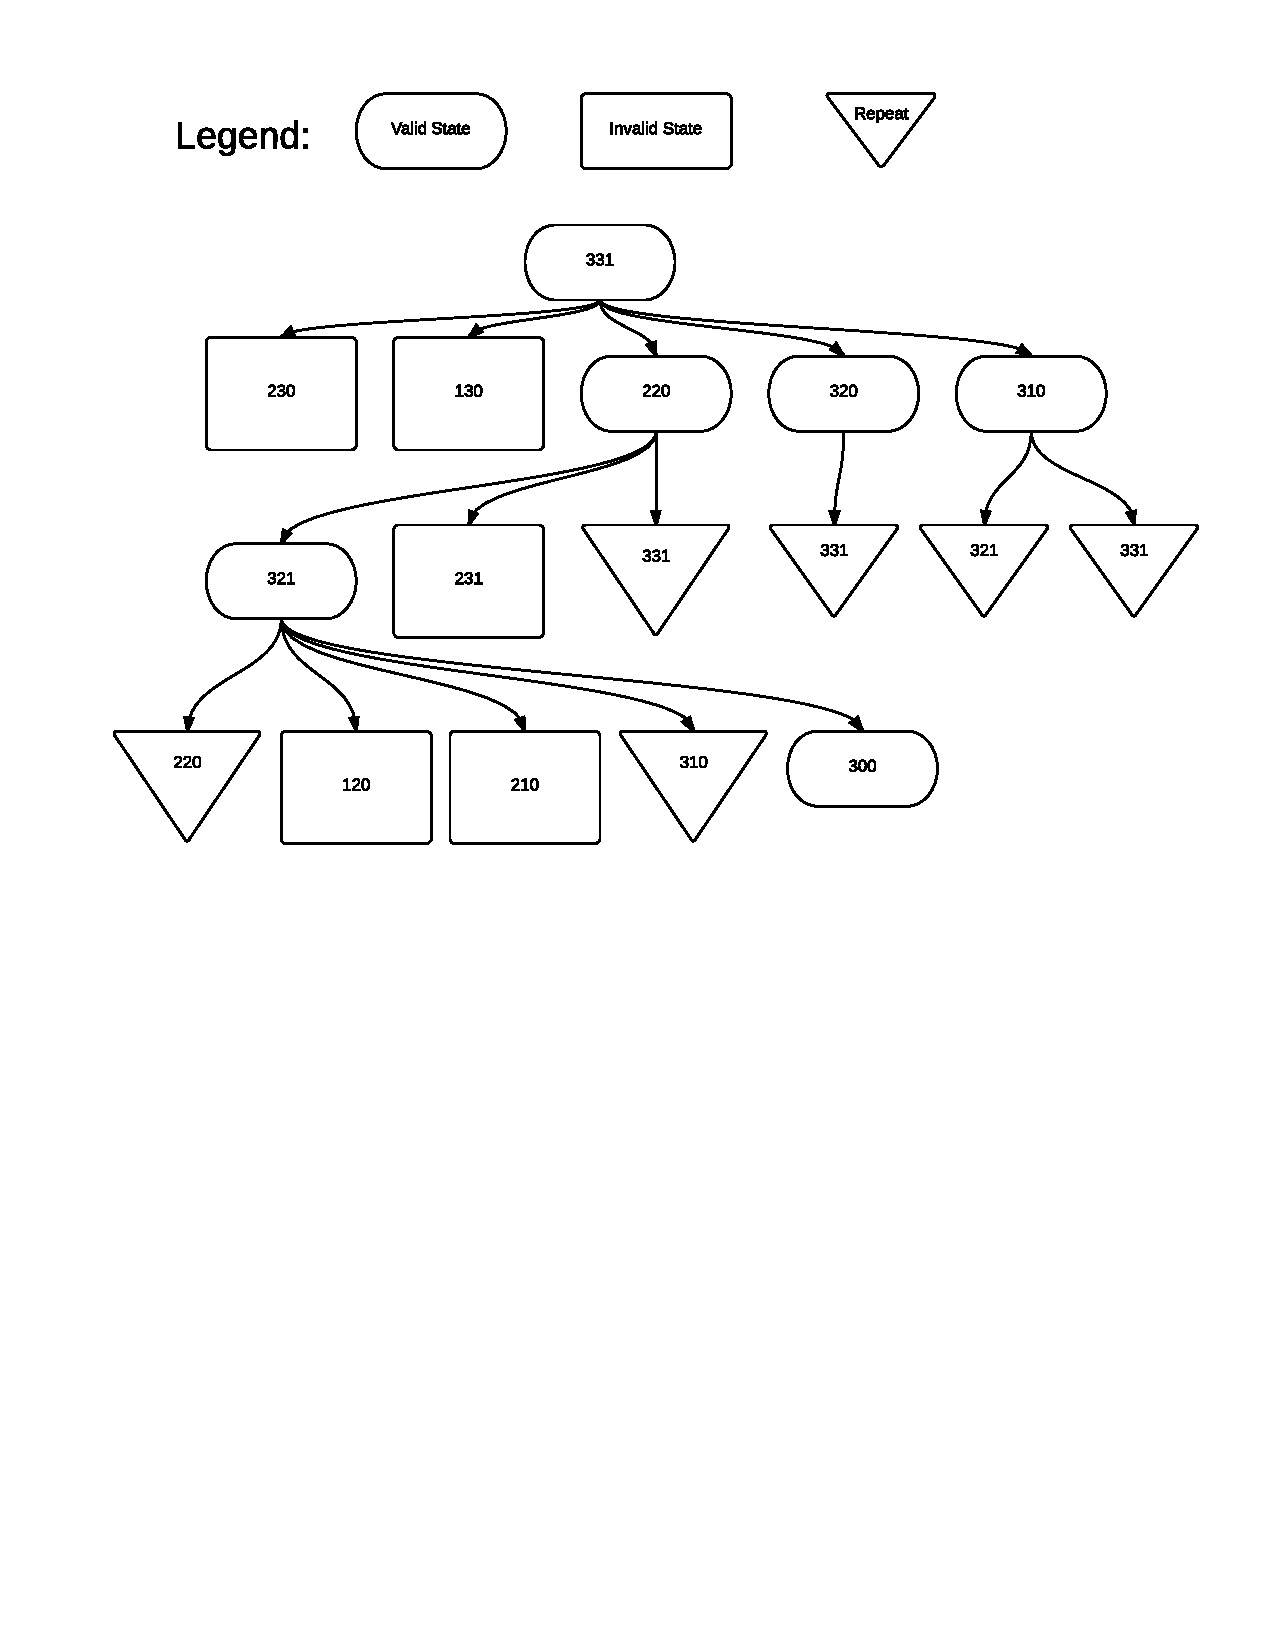
\includegraphics{drawing.pdf}


\section{Implementation of the model}
%Present the work in your report. Include the key parts of your code using the listings environment in LaTeX, and discuss how the code works. 
%Also describe your testing and convince the reader that your testing process demonstrated correctness of your code.
The model is implemented in 
\verb`CannibalProblem.java`.  Here's my code for \verb`getSuccessors`:

\begin{lstlisting}
public ArrayList<UUSearchNode> getSuccessors() {
  // the final array to be returned
  ArrayList<UUSearchNode> retArr = new ArrayList<UUSearchNode>();
  
  int boatPlace = state[2];
  int candMissionaries = -1;
  int candCannibals = -1;
  int candBoat = -1;
  
  // Determine which missionaries and cannibals can travel
  if (boatPlace == 1){
    System.out.println("Boat @ starting side");
    // the candidate missionaries that can travel on the boat
    candMissionaries = state[0];
    candCannibals = state[1];
    candBoat = 0;
  } else if (boatPlace == 0){
    candMissionaries = totalMissionaries - state[0];
    candCannibals = totalCannibals - state[1];
    candBoat = 1;
  } else {
    // not valid input for boat
    System.out.println("Boat place not valid: " + boatPlace);
    System.exit(1);
  }
  
  for(int missCount=candMissionaries; missCount>=0; missCount--){
    for(int cannCount=candCannibals; cannCount>=0; cannCount--){
      System.out.println("Checking ("+missCount+","+cannCount+")");
      CannibalNode possNode;
      
      // Must fit in boat and have at least one missionary rowing
      if (missCount + cannCount <= BOAT_SIZE && (missCount > 0 || cannCount > 0)){
        // Must have something happen
        if (missCount == 0 && cannCount == 0){
          continue;
        }
        
        if (boatPlace == 1){
          // boat on starting side so starting side is subtracted
          possNode = new CannibalNode(candMissionaries - missCount, 
              candCannibals - cannCount, candBoat, depth+1);
        } else {
          // boat on other side so starting side is added
          possNode = new CannibalNode( state[0] + missCount, 
              state[1] + cannCount, candBoat, depth+1);
        }
        System.out.println("("+possNode.state[0]+","+possNode.state[1]+","+possNode.state[2]+")");
      } else {
        continue;
      }
      
      boolean isSafe = isSafeState(possNode);
      if (isSafe){
        // State is valid, add to the array
        System.out.println("Adding " + possNode);
        retArr.add(possNode);
      } else {
        // Node was not a valid state
        System.out.println("Not a safe state!");
      }
    }
  }
  return retArr;
}
\end{lstlisting}

The basic idea of \verb`getSuccessors` is that it returns an array of valid states
based off of the node that was passed in. So, given the first start node: (331), it will
run through each combination of missionaries and cannibals. So it checks 3 Missionaries and 
3 Cannibals on the boat, then 3 Missionaries 2 Cannibals, then 3 Missionaries 1 Cannibal, 
3 Missionaries 0 Cannibals, 2 Missionaries 1 Cannibal and so on. As per the drawing before,
the valid states from a $getSuccessors$ on (331) are: (220), (320), (310).

Then, it will check if 
that combination is valid for the boat size. Also check whether there is anybody on the
boat itself to mark whether the edge is valid or not. If it is, it will add or subtract (depending
on where the boat is) to create the new state. This new state is passed into the \verb`isSafeState`
to verify whether the missionaries are safe. If they are, return true. If not, return false.


\begin{lstlisting}
// checks whether the humans get eaten :(
private boolean isSafeState(CannibalNode node){
  // miss + cannibals on starting side
  int startMissionaries = node.state[0];
  int startCannibals = node.state[1];
  // miss + cannibals on other side
  int otherMissionaries = totalMissionaries - startMissionaries;
  int otherCannibals = totalCannibals - startCannibals;
  
  if (startMissionaries != 0 && otherMissionaries != 0){
    // must have more missionaries than cannibals or else eaten :(
    if (startMissionaries >= startCannibals && 
        otherMissionaries >= otherCannibals){
      return true;
    }
  }
  
  // If no missionaries are on one side, must mean missionaries are on other side
  // Therefore, we check if the missionaries are outnumbered on the other side
  // Also starting with 1 Cannibal and 0 Missionaries on starting side is NOT 
  // a valid state
  if (otherMissionaries == 0){
    return startMissionaries >= startCannibals;
  }
  
  if (startMissionaries == 0){
    return otherMissionaries >= otherCannibals;
  }
  
  // not a safe state
  return false;
}

\end{lstlisting}

I used a method \verb`isSafeState` that returns \verb`true` if the missionaries do not get
eaten by the cannibals. We can check this by first validating that there are missionaries on
either side of the river. Then we MUST make sure that the cannibals cannot outnumber
missionaries on either side. 

If there are no missionaries on one side, that implies that all the missionaries are on the 
other side. Thus, we just need to check whether the missionaries are outnumbered on the other side. 
This will cover the edge case where there are no missionaries but more than 0 cannibals on the same side. 
Without this edge case, the algorithm would not correctly process a node like (031).

Overall, I tested both methods by manually expanding the states graph from the initial problem setup of
(331) and then cross-checking with the results that the \verb`getSuccessors` method yields. This verifies
the method for the first level. We could test the second and third levels in the states graph via grabbing
the array returned by the first \verb`getSuccessors` method and calling \verb`getSuccessors` again on 
one of the valid states.

Below is the code for a private method in $CannibalProblem.java$ and some manual code executed in 
$CannibalDriver.java$. 

\begin{lstlisting}
private void testSuccessors(){
  ArrayList<UUSearchNode> retArr = startNode.getSuccessors();
  System.out.println(retArr);
}
\end{lstlisting}

\begin{lstlisting}
// Test levels 2 and 3
ArrayList<UUSearchNode> retArr = mcProblem.startNode.getSuccessors();
System.out.println(retArr.get(0).getSuccessors().get(1).getSuccessors());
\end{lstlisting}

Since the code works for levels 1, 2 and 3 and matches the actual valid states drawn manually, 
it covers the the cases for the boat going from one side to another. In other words, given an arbitrary
state at level x, we get the valid successor states for state x+1 level. Thus, by induction, we prove
the correctness of the code. We cross-reference with the drawing above to verify the states returned
are valid states. 

Hence the $getSuccessors()$ and $isSafeState()$ methods are correct. 

\section{Breadth-first search}
\begin{lstlisting}
public List<UUSearchNode> breadthFirstSearch(){
  resetStats();
  
  // Goal node that completes the search
  UUSearchNode goalNode = null;
  UUSearchNode grandparent = null;
  
  // Initialize queue with start node
  Queue<UUSearchNode> queue = new LinkedList<UUSearchNode>();
  queue.add(startNode);
  HashMap<Integer, UUSearchNode> visited = new HashMap<Integer, UUSearchNode>();
  
  while(!queue.isEmpty()){
    updateMemory(queue.size() + visited.size());
    System.out.println("Queue: " + queue);
    UUSearchNode parentNode = (UUSearchNode) queue.remove();
    System.out.println("Using " + parentNode);
    
    incrementNodeCount();
    
    // check if the goal has been reached
    if (parentNode.goalTest()){
      goalNode = parentNode;
      int key = parentNode.hashCode();
      visited.put(key, grandparent);
      break;
    }
    
    ArrayList<UUSearchNode> children = parentNode.getSuccessors();
    for(int i=0; i < children.size(); i++){
      // if haven't seen before
      UUSearchNode childNode = children.get(i);
      int nodeKey = childNode.hashCode();
      System.out.println(nodeKey);
      if (!visited.containsKey(nodeKey)){
        // mark previous node 
        if (!queue.contains(childNode)){
          queue.add(childNode);
        }
      } else {
        System.out.println("Already seen " + childNode);
      }
    }
    // visited 'key' will contain the hashCode of the node 
    // visited 'value' will contain the node's predecessor node 
    // startNode has no predecessor
    int key = parentNode.hashCode();
    visited.put(key, grandparent);
    
    // once all children have been added, mark this node visited
    grandparent = parentNode;
    
  }
  
  
  System.out.println(goalNode);
  
  // Check if goalNode has been found
  if (goalNode == null){
    return null;
  } else {
    // return the backchain link
    return backchain(goalNode, visited);
  }
}

// backchain should only be used by bfs, not the recursive dfs
private List<UUSearchNode> backchain(UUSearchNode goalNode,
    HashMap<Integer, UUSearchNode> visited) {
  List<UUSearchNode> retArr = new ArrayList<UUSearchNode>();
  while (goalNode != null){
    retArr.add(goalNode);
    goalNode = visited.get(goalNode.hashCode());
  }
  return retArr;
}
\end{lstlisting}
%Test, present, and discuss your code in the report.
%A good test would at the very least check the breadth-first search with respect to the nodes you drew in the intro.
%Show the solution output by your code for missionaries and cannibals.

We implement BFS with a queue and a HashMap (instead of a linked list which is not as efficient). 
The queue is FIFO and allows us to dequeue the startNode and enqueue its successors, then dequeue the
first level of the startNode's successors and enqueue $their$ successors etc. By nature of BFS, we 
successively check each depth level from the startNode. We also avoid duplicates by checking if
the queue already contains some node. 

The HashMap visited will keep track of which nodes have already been 
visited by using the provided $hashCode$ function. The key of the HashMap is the hashcode of the node. 
The value of the HashMap is the predecessor node that links to it in the graph. We track the memory by considering the size of the queue
and the size of the $visited$ HashMap at any point. We also increment the nodes count each time we dequeue a node
from the queue. 

Thus, when we find the goalnode, we can simply use a 
$while$ loop to backchain from goalnode using the $visited$ HashMap to find its predecessor. 

If no path is found, we return $null$. Otherwise, return the path via backchaining. 

% testing %
We test the BFS by running on state (331) and verifying that states are valid and that the path from start node to
goal node make valid action edges. 

\begin{lstlisting}
List<UUSearchProblem.UUSearchNode> path;
path = mcProblem.breadthFirstSearch();	

if (path != null){
  System.out.println("bfs path length:  " + path.size() + " " + path);
  mcProblem.printStats();
  System.out.println("--------");
} else {
  System.out.println("--------");
  System.out.println("No path!");
}
\end{lstlisting}

% solution output %
The solution path, including the start node, is of length 15:

\begin{lstlisting}
bfs path length:  15 [0, 0, 0, (11)|, 0, 2, 1, (10)|, 1, 1, 1, (10)|,
0, 1, 0, (9)|, 0, 3, 1, (8)|, 0, 2, 0, (7)|, 2, 2, 1, (6)|, 
1, 1, 0, (5)|, 3, 1, 1, (4)|, 3, 0, 0, (3)|, 3, 2, 1, (2)|, 
3, 2, 0, (1)|, 3, 1, 0, (1)|, 2, 2, 0, (1)|, 3, 3, 1, (0)|]
Nodes explored during last search:  15
Maximum memory usage during last search 15
\end{lstlisting}

We can manually verify that all the states are correctly reached through valid actions by actually tracing
each iteration of the 2 $for$ loops in the $getSuccessors()$ method. Then checking the path that BFS takes (it should
explore each node in a depth first before continuing to the next depth). 
\begin{lstlisting}
Queue: [3, 3, 1, (0)|]
Using 3, 3, 1, (0)|
(1,3,0)
Not a safe state!
(2,2,0)
Adding 2, 2, 0, (1)|
(2,3,0)
Not a safe state!
(3,1,0)
Adding 3, 1, 0, (1)|
(3,2,0)
Adding 3, 2, 0, (1)|
Queue: [2, 2, 0, (1)|, 3, 1, 0, (1)|, 3, 2, 0, (1)|]
Using 2, 2, 0, (1)|
(3,3,1)
Adding 3, 3, 1, (2)|
(3,2,1)
Adding 3, 2, 1, (2)|
(2,3,1)
Not a safe state!
Already seen 3, 3, 1, (2)|
Queue: [3, 1, 0, (1)|, 3, 2, 0, (1)|, 3, 2, 1, (2)|]
Using 3, 1, 0, (1)|
(3,3,1)
Adding 3, 3, 1, (2)|
(3,2,1)
Adding 3, 2, 1, (2)|
Already seen 3, 3, 1, (2)|
Queue: [3, 2, 0, (1)|, 3, 2, 1, (2)|]
Using 3, 2, 0, (1)|
(3,3,1)
Adding 3, 3, 1, (2)|
Already seen 3, 3, 1, (2)|
Queue: [3, 2, 1, (2)|]
Using 3, 2, 1, (2)|
(1,2,0)
Not a safe state!
(2,1,0)
Not a safe state!
(2,2,0)
Adding 2, 2, 0, (3)|
(3,0,0)
Adding 3, 0, 0, (3)|
(3,1,0)
Adding 3, 1, 0, (3)|
Already seen 2, 2, 0, (3)|
Already seen 3, 1, 0, (3)|
Queue: [3, 0, 0, (3)|]
Using 3, 0, 0, (3)|
(3,2,1)
Adding 3, 2, 1, (4)|
(3,1,1)
Adding 3, 1, 1, (4)|
Already seen 3, 2, 1, (4)|
Queue: [3, 1, 1, (4)|]
Using 3, 1, 1, (4)|
(1,1,0)
Adding 1, 1, 0, (5)|
(2,0,0)
Not a safe state!
(2,1,0)
Not a safe state!
(3,0,0)
Adding 3, 0, 0, (5)|
Already seen 3, 0, 0, (5)|
Queue: [1, 1, 0, (5)|]
Using 1, 1, 0, (5)|
(3,1,1)
Adding 3, 1, 1, (6)|
(2,2,1)
Adding 2, 2, 1, (6)|
(2,1,1)
Not a safe state!
(1,3,1)
Not a safe state!
(1,2,1)
Not a safe state!
Already seen 3, 1, 1, (6)|
Queue: [2, 2, 1, (6)|]
Using 2, 2, 1, (6)|
(0,2,0)
Adding 0, 2, 0, (7)|
(1,1,0)
Adding 1, 1, 0, (7)|
(1,2,0)
Not a safe state!
(2,0,0)
Not a safe state!
(2,1,0)
Not a safe state!
Already seen 1, 1, 0, (7)|
Queue: [0, 2, 0, (7)|]
Using 0, 2, 0, (7)|
(2,2,1)
Adding 2, 2, 1, (8)|
(1,3,1)
Not a safe state!
(1,2,1)
Not a safe state!
(0,3,1)
Adding 0, 3, 1, (8)|
Already seen 2, 2, 1, (8)|
Queue: [0, 3, 1, (8)|]
Using 0, 3, 1, (8)|
(0,1,0)
Adding 0, 1, 0, (9)|
(0,2,0)
Adding 0, 2, 0, (9)|
Already seen 0, 2, 0, (9)|
Queue: [0, 1, 0, (9)|]
Using 0, 1, 0, (9)|
(2,1,1)
Not a safe state!
(1,2,1)
Not a safe state!
(1,1,1)
Adding 1, 1, 1, (10)|
(0,3,1)
Adding 0, 3, 1, (10)|
(0,2,1)
Adding 0, 2, 1, (10)|
Already seen 0, 3, 1, (10)|
Queue: [1, 1, 1, (10)|, 0, 2, 1, (10)|]
Using 1, 1, 1, (10)|
(0,0,0)
Adding 0, 0, 0, (11)|
(0,1,0)
Adding 0, 1, 0, (11)|
(1,0,0)
Not a safe state!
Already seen 0, 1, 0, (11)|
Queue: [0, 2, 1, (10)|, 0, 0, 0, (11)|]
Using 0, 2, 1, (10)|
(0,0,0)
Adding 0, 0, 0, (11)|
(0,1,0)
Adding 0, 1, 0, (11)|
Already seen 0, 1, 0, (11)|
Queue: [0, 0, 0, (11)|]
Using 0, 0, 0, (11)|
0, 0, 0, (11)|
\end{lstlisting}


The above sequence validates BFS is working correctly and taking the correct paths
for the problem of (331). 

\section{Memoizing depth-first search}
\begin{lstlisting}
public List<UUSearchNode> depthFirstMemoizingSearch(int maxDepth) {
  resetStats(); 
  
  // You will write this method
  List<UUSearchNode> retArr = new ArrayList<UUSearchNode>();
  HashMap<UUSearchNode, Integer>visited = new HashMap<UUSearchNode, Integer>();
  
  List<UUSearchNode> startChildren = startNode.getSuccessors();
  
  // mark startNode as visited
  visited.put(startNode, startNode.getDepth());

  for(int i=0; i < startChildren.size(); i++){
    UUSearchNode child = startChildren.get(i);
    if (!visited.containsKey(child)){
      retArr = dfs(child, visited, child.getDepth(), CannibalDriver.MAXDEPTH);
      if (retArr != null){
        return retArr;
      }
    }
    
  }
  return null;
}

// recursive memoizing dfs. Private, because it has the extra
// parameters needed for recursion.  
private List<UUSearchNode> dfs(UUSearchNode currentNode, HashMap<UUSearchNode, Integer> visited, 
    int depth, int maxDepth) {
  System.out.println("Following " + currentNode);
  
  // keep track of stats; these calls charge for the current node
  updateMemory(visited.size());
  incrementNodeCount();
  List<UUSearchNode> retArr= new ArrayList<UUSearchNode>();

  // you write this method.  Comments *must* clearly show the 
  //  "base case" and "recursive case" that any recursive function has.	
  
  // BASE CASE: currentNode is the goal Node
  if (currentNode.goalTest()){
    retArr.add(currentNode);
    return retArr;
  } else {
    // RECURSIVE CASE: not the goalNode, continue recursing down successor line
    List<UUSearchNode> currentChildren = currentNode.getSuccessors();
    visited.put(currentNode, currentNode.getDepth());
    
    // stop if the depth is exceeded
    if (depth > maxDepth){
      System.out.println("Depth exceeded! Try a shorter route");
      return null;
    }
    
    for(int i=0; i < currentChildren.size(); i++){
      UUSearchNode child = currentChildren.get(i);
      
      // if it is depth limited, we need to make sure that the DFS doesn't stop at 
      // a duplicate (compare depths)
      if (!visited.containsKey(child) || visited.get(child) > depth){
        retArr = dfs(child, visited, child.getDepth(), maxDepth);
        if (retArr != null){
          retArr.add(child);
          return retArr;
        }
      } 
    }
  System.out.println("No path found!");
    return null;
  }
  
}

\end{lstlisting}
%Every recursive algorithm has at least one base case and at least one recursive case. What are they for this problem? Present and discuss your code, clearly labelling the base cases and the recursive cases.
We start by initializing the array which will be returned as the solution. We also initialize the HashMap which will
mark whether the node has been visited and will have the key as the depth. We add the depth because, in some cases, 
if one sets a MAX DEPTH for DFS, DFS may explore one path and exceed this max depth. Then, when DFS checks shorter
paths, it may run into a duplicate. We want DFS to continue if this duplicate's depth is smaller than the original node's
depth. Hence, we add the $visited.get(child) > depth$ method in the recursive DFS method.

The base case for memoizing DFS is if the node being examined is the goal node. In that case, we do not enter the recursive case and we can simply add this goal node into a list
and return it.

The recursive case is if the node being examined is NOT the goal node. We also make checks so that the depth does not 
exceed $maxDepth$. 

We loop through each one of the $startNode$'s successors and then run the recursive DFS method on them. In the
recursive DFS function, if the node has already been seen, we return $null$. If the node has not been seen,
we run recursive DFS again on each of the node's successors.

When the goal node is finally reached, as said before, we add it to a list and return that list. Then in the
recursive DFS function, if the returned list is NOT $null$, then we add the currently examined node to that list
and return the expanded list. In this way, we build the solution from the ground-up, starting with the
goal node and then progressively adding nodes that link to one another.

%Does memoizing dfs save significant memory with respect to breadth-first search? Why or why not?
However, memoizing dfs does NOT save significant memory compared to BFS. First, we consider whether the state space is finite or infinite. 
Given a finite state space of size $n$, the HashMap implemented in both DFS and BFS cannot exceed $n$ nodes at any given time. Thus,
both BFS and DFS implementations in the finite search space have $O(n)$ memory usage. Thus, they have the same $O(n)$ memory usage
although DFS may have $slightly$ lower memory usage compared to BFS if we find the goal soon and the $visited$ set is small. 
But if one finds the goal late, memory usage will be higher. In contrast, BFS goes through each depth successively. 

However, by nature of BFS, because it ripples out from the
start node and checks each successive depth from the start node, in an infinite state space, BFS will terminate with time complexity $O(b^d)$, 
where $d$ is the depth of the goal from start node and $b$ is the upper bound of the graph's branching factor. 

Conversely, in an infinite search space, DFS may not even terminate (without a MAXDEPTH limit)! Hence, in some cases, DFS may have substantially more exhaustive
memory usage. However, as in the case of (331), it is possible for DFS to find the optimal path in the first ``go'' without backchaining. 
Thus, in these rare scenarios, could save some memory. 

However, this is not consistent. Furthermore, DFS does not guarantee an optimal path if the goal is close. Thus, one should not use
memoizing DFS over BFS unless one has a very good reason to do so: 

\begin{lstlisting}
List<UUSearchProblem.UUSearchNode> path;
path = mcProblem.depthFirstMemoizingSearch(MAXDEPTH);	
if (path != null){
  System.out.println("dfs memoizing path length:" + path.size());
  mcProblem.printStats();
  System.out.println("--------");
}

dfs memoizing path length:11
Nodes explored during last search:  11
Maximum memory usage during last search 11
\end{lstlisting}

\begin{lstlisting}
(1,3,0)
Not a safe state!
(2,2,0)
Adding 2, 2, 0, (1)|
(2,3,0)
Not a safe state!
(3,1,0)
Adding 3, 1, 0, (1)|
(3,2,0)
Adding 3, 2, 0, (1)|
Following 2, 2, 0, (1)|
(3,3,1)
Adding 3, 3, 1, (2)|
(3,2,1)
Adding 3, 2, 1, (2)|
(2,3,1)
Not a safe state!
Following 3, 2, 1, (2)|
(1,2,0)
Not a safe state!
(2,1,0)
Not a safe state!
(2,2,0)
Adding 2, 2, 0, (3)|
(3,0,0)
Adding 3, 0, 0, (3)|
(3,1,0)
Adding 3, 1, 0, (3)|
Following 3, 0, 0, (3)|
(3,2,1)
Adding 3, 2, 1, (4)|
(3,1,1)
Adding 3, 1, 1, (4)|
Following 3, 1, 1, (4)|
(1,1,0)
Adding 1, 1, 0, (5)|
(2,0,0)
Not a safe state!
(2,1,0)
Not a safe state!
(3,0,0)
Adding 3, 0, 0, (5)|
Following 1, 1, 0, (5)|
(3,1,1)
Adding 3, 1, 1, (6)|
(2,2,1)
Adding 2, 2, 1, (6)|
(2,1,1)
Not a safe state!
(1,3,1)
Not a safe state!
(1,2,1)
Not a safe state!
Following 2, 2, 1, (6)|
(0,2,0)
Adding 0, 2, 0, (7)|
(1,1,0)
Adding 1, 1, 0, (7)|
(1,2,0)
Not a safe state!
(2,0,0)
Not a safe state!
(2,1,0)
Not a safe state!
Following 0, 2, 0, (7)|
(2,2,1)
Adding 2, 2, 1, (8)|
(1,3,1)
Not a safe state!
(1,2,1)
Not a safe state!
(0,3,1)
Adding 0, 3, 1, (8)|
Following 0, 3, 1, (8)|
(0,1,0)
Adding 0, 1, 0, (9)|
(0,2,0)
Adding 0, 2, 0, (9)|
Following 0, 1, 0, (9)|
(2,1,1)
Not a safe state!
(1,2,1)
Not a safe state!
(1,1,1)
Adding 1, 1, 1, (10)|
(0,3,1)
Adding 0, 3, 1, (10)|
(0,2,1)
Adding 0, 2, 1, (10)|
Following 1, 1, 1, (10)|
(0,0,0)
Adding 0, 0, 0, (11)|
(0,1,0)
Adding 0, 1, 0, (11)|
(1,0,0)
Not a safe state!
Following 0, 0, 0, (11)|
\end{lstlisting}


\section{Path-checking depth-first search}
% Write it. Present it. Discuss it. %

In Path-checking DFS, we ensure that the current path does not contain duplicates by using a set, currentPath. As a result,
we avoid infinite loops. Each time we're about to call $getSuccessors()$ on a child node, we check the set
to ensure that it has not already been added. Thus, we don't track all states once, just the ones on the 
current path. 

This only ensures that there are no duplicates in the $current$ path, but we could run into redundant 
nodes in other paths. The benefit, however, is that we use less memory than simply memoizing everything
as in the previous memoizing DFS. 

\begin{lstlisting}
// set up the depth-first-search (path-checking version), 
//  but call dfspc to do the real work
public List<UUSearchNode> depthFirstPathCheckingSearch(int maxDepth) {
  resetStats();
  
  // I wrote this method for you.  Nothing to do.
  HashSet<UUSearchNode> currentPath = new HashSet<UUSearchNode>();

  return dfsrpc(startNode, currentPath, 0, maxDepth);
}

// recursive path-checking dfs. Private, because it has the extra
// parameters needed for recursion.
private List<UUSearchNode> dfsrpc(UUSearchNode currentNode, HashSet<UUSearchNode> currentPath,
    int depth, int maxDepth) {

  // you write this method
  System.out.println("Following " + currentNode);
  currentPath.add(currentNode);
  
  // keep track of stats; these calls charge for the current node
  updateMemory(currentPath.size());
  incrementNodeCount();
  List<UUSearchNode> retArr= new ArrayList<UUSearchNode>();

  // you write this method.  Comments *must* clearly show the 
  //  "base case" and "recursive case" that any recursive function has.	
  
  // BASE CASE: currentNode is the goal Node
  if (currentNode.goalTest()){
    retArr.add(currentNode);
    return retArr;
  } else {
    // RECURSIVE CASE: not the goalNode, continue recursing down successor line
    List<UUSearchNode> currentChildren = currentNode.getSuccessors();
    
    // stop if the depth is exceeded
    if (depth > maxDepth){
      System.out.println("Depth exceeded! Try a shorter route");
      return null;
    }
    
    for(int i=0; i < currentChildren.size(); i++){
      UUSearchNode child = currentChildren.get(i);
      
      // if it is depth limited, we need to make sure that the DFS doesn't stop at 
      // a duplicate (compare depths)
      if (!currentPath.contains(child)){
        retArr = dfsrpc(child, currentPath, child.getDepth(), maxDepth);
        if (retArr != null){
          retArr.add(child);
          return retArr;
        }
      } 
    }
    return null;
  }

}
\end{lstlisting}

% Does path-checking depth-first search save significant memory with respect to breadth-first search?  
It depends on the graph that path-checking DFS and BFS are run, but generally path-checking does save
a lot of memory given a looping graph. 
BFS could store all the nodes on the graph in its $visited$ set so that its memory cost is
$n$ nodes. In this situation, path-checking's $currentPath$ only stores the nodes found in the current path. 
The current path to the goalNode could only contain a small fraction of such nodes and save significant amounts
of memory. While the memory allocated still needs to accomodate $n$ nodes because hypothetically the $currentPath$ set
could contain $n$ nodes, on average, depending on the graph, significant memory could be saved via path-checking. 

However, the trade-off, as said before, is that one may run into redundant paths and increase the runtime of
the path-checking DFS. This is a potential cost of nodes being visited twice. 

% Draw an example of a graph where path-checking dfs takes much more run-time than breadth-first search; 
% include in your report and discuss. 
Path-checking DFS may face a graph with many non-looping paths. Then it will check redundant paths over and over.
Consider the following example where path-checking DFS takes much more run-time than BFS:

\hspace*{-2in}
\includegraphics{path_dfs.pdf}

In this graph, path-checking BFS will separately check 3 branches of B-C-D in the runtime. In contrast, BFS will check
the B node first, then skip the other 2 B nodes and arrive at G. Thus, path-checking BFS faces a graph with many 
non-loops and traverses many redundant paths. Hence, it takes much more runtime than BFS, especially if the branching factor
of such non-loop paths is high. 

\section{Iterative deepening search}

\begin{lstlisting}
public List<UUSearchNode> IDSearch(int maxDepth) {
  resetStats();
  for(int i=0; i <= maxDepth; i++){
    HashMap<UUSearchNode, Integer> visited = new HashMap<UUSearchNode, Integer>();
    List<UUSearchNode> retArr = dfs(startNode, visited, 0, maxDepth);
    if (retArr != null){
      return retArr;
    }
  }
  System.out.println("No path found!");
  return null;
}
\end{lstlisting}

% On a graph, would it make sense to use path-checking dfs, 
% or would you prefer memoizing dfs in your iterative deepening search? 
% Consider both time and memory aspects. (Hint. If it's not better than bfs, just use bfs.)
BFS finds the shortest path because it goes from smallest depth to longest. Iterative deepening search
mimics this by restricting the DFS to depth 0 at first and then slowly incrementing the depth when it doesn't
find the goal. So if the goal is at layer 3, IDS will do DFS on all paths at level depth 0, then depth 1, then
depth 2, and finally at depth 3 where it finds the goal. 
If IDS does find the goal, then that goal is optimal because we do not check any nodes deeper than the goal depth. 

IDS does not take huge amounts of memory as its requisite memory is bound by maxdepth. To see why, consider the longest paths. 
The longest path in layer 1 is 1. The longest path in layer 2 is 2. Thus, the longest path is bounded by the 
maximum depth provided in IDS. Thus, we can check layer 1, then dump the memory information if goal is not found.
And continue doing the same for the next layers. 

IDS's runtime is not worse than BFS as the max depth is limited as well. The IDS's most expensive DFS will be about the same
as BFS's worst case. Thus, it is very efficient. One scenario where IDS could be slow is if the graph has many branches
at each depth. 

Whether I would prefer memoizing DFS or path-checking DFS would depend on the graph I am searching. If the graph has many
branches in each of its depths and many redundant nodes in such paths, memoizing may be a good idea. It would prevent duplication
of effort at the expense of more memory. However, IDS with memoizing would not be better than BFS, so I would simply revert to 
BFS. 

If the graph has many loops in its current paths at each depth, path-checking DFS would be a good idea as it would use
less memory and have roughly the same runtime because there is little duplication of effort given that we assume
few redundant paths.  In this situation, path-checking with IDS would save on memory compared to BFS as BFS memoizes all states
that have been visited. 


\section{Lossy missionaries and cannibals}
% What would the state for this problem be? 
We can still define the state of the lossy missionaries and cannibals problem with (m, c, b) where
$m$ is the number of missionaries, $c$ is the number of cannibals and $b$ is the side that the boat 
is on. Hence, given the original problem with $E$ missionaries willing to be eaten, we can still define
the problem as (3, 3, 1). 

% What changes would you have to make to your code to implement a solution? 
To implement the concept of ``lossy'' missionaries, we can define the static constant $E$ in the
CannibalDriver.java, as we did with the MAX DEPTH constant. Then, we would simply modify $isSafeState()$
function. 

We can modify the $if$ statement in $isSafeState()$ where in the original problem, checks whether there are more cannibals than
missionaries. With $E$ missionaries now willing to die, we can check whether the side opposite of the boat 
has $E$ or less missionaries.

If so, it will be safe to send any number of cannibals to that side (with 0 missionaries). Or send any number of missionaries
with cannibals to that side such that the total number of resultant missionaries (when the boat arrives) is still less than
$E$.

An $if$ statement like this would work: 

\begin{lstlisting}
  if (startMissionaries + missionariesSent <= E && boatPlace == 0){
    return true;
  }
\end{lstlisting}

Or conversely, for the other side:

\begin{lstlisting}
  if (otherMissionaries + missionariesSent <= E && boatPlace == 1){
    return true;
  }
\end{lstlisting}

We would also need to keep track of how many missionaries have been eaten already, perhaps through a variable
called $eatenCount$. We use this variable in order to calculate the missionaries on the other side. For instance if
$eatenCount == 2$, then if the current state is at $(1,1,0)$. Given the original problem, then we know that are 0
missionaries on the other side and 2 cannibals on the other side. 


% Give an upper bound on the number of possible states for this problem.
The total upper bound for valid and invalid states is the same. For the given 3 missionaries, 3
cannibals and boat on starting side, the total number of valid/invalid states is still $4 \cdot 4 \cdot 2$.



\end{document}
